\section{Résultats}

Enfin, le spectre de puissance Ly-$\alpha$ observé par BOSS est ajusté par cette série de paramètre grâce au logiciel \textsf{MUNUIT}~\cite{Minuit}, ainsi qu'un total de 27 paramètres de nuisance qui corrigent les spectres produits numériquement par la résolution du spectrographe, le niveau de bruit dans chaque bin en redshift, la corrélation entre les transitions Ly-$\alpha$, Si\textsc{ii} et Si\textsc{iii}, modélisation de certains mécanismes de contre-réactions \textit{etc}. Ceux-ci sont tous décrit dans \cite{Palanque2015a, Palanque2015b, Baur16}. Le package \textsf{MINUIT} identifie le meilleur ajustement à partir du minimum du $\chi^2$ évalué en laissant libres tous les paramètres dans la table \ref{tab:parametres} et les paramètres de nuisance. L'intervalle de vraisemblance (CL) d'un des $n$ paramètres $\theta_i$ est calculé en minimisant le $\chi2$ en fixant chacun des $n-1$ paramètres restants. Pour les intervalles à 2 dimensions, les $n-2$ paramètres sont fixés et le $\chi^2$ est évalué en scannant les valeurs de $(\theta_i, \theta_j)$. En supposant que toutes les erreurs expérimentales sont distribuées normalement, \\
\begin{equation}
\mathrm{CL}(\theta_i, \theta_j, ..., \theta_n) = 1 - \int_{\Delta \chi^2 (\theta_i, \theta_j, ..., \theta_n)}^{\infty} \mathrm{d} x ~ f_{N_{\mathrm{dof}}}(x)
\end{equation} \\ où la fonction de distribution pour $N_\mathrm{dof}$ degrées de liberté est \\
\begin{equation}
f_{N_{\mathrm{dof}}}(x) ~ = ~ \frac{e^{-x/2} ~ x^{\frac{N_{\mathrm{dof}}}{2}-1}}{\sqrt{2^{N_{\mathrm{dof}}}} ~ \Gamma (N_{\mathrm{dof}}/2)}
\end{equation} \\ et $\Gamma (z) = \displaystyle \int_{0}^{\infty} \mathrm{d}x~ x^{z-1} e^{-x}$ est la fonction gamma. Les intervalles de vraisemblance à $1\sigma$, $2\sigma$ et $3\sigma$ sur $\theta_i$ ou ($\theta_i$, $\theta_j$) correspondent à une valeur du $\chi^2$ de $\Delta \chi^2 (\theta_i) = 1, 4$ et $9$ and $\Delta \chi^2 (\theta_i, \theta_j) = 2.30, 6.18$ et $11.83$ respectivement, par rapport à la valeur extrêmale $\chi^2_\mathrm{min}$. \\

\begin{table}
\begin{center}
\begin{tabular}{lcc}
\hline \\[-10pt]
\textbf{paramètre} & \multicolumn{2}{c}{\textbf{Ly-$\alpha$ + $H_0$}} \\[2pt]
 & \textbf{SDSS/BOSS DR9} & \textbf{SDSS + XQ-100}\\[2pt]
\hline \\[-10pt]
\\ [2pt]
$h$ & $0.673 \pm 0.010$ & $0.671 \pm 0.010$ \\[2pt]
$\Omega_m$ & $0.293 \pm 0.014$ & $0.279 \pm 0.011$ \\[2pt]
$\sigma_8$ & $0.831 \pm 0.031$ & $0.797 \pm 0.023$ \\[2pt]
$n_s$ & $0.939 \pm 0.010$ & $0.956 \pm 0.007$ \\[2pt]
%\hline \\[-10pt]
%$d n_s / d \ln k$ & . & . \\[2pt]
%$N_{\mathrm{eff}}$ & . & . \\[2pt]
\hline \\[-10pt]
%$z_\star$ & . & . \\[2pt]
$T_0^{z=3}/10^3\mathrm{K}$ & $8.9^{+3.8}_{-4.0}$ & $12.8 \pm 3.1$ \\[2pt]
$\eta^{T_0}_{z<3}$ & $-2.9 \pm 0.5$ & $-2.0 \pm 0.5$ \\[2pt]
$\eta^{T_0}_{z>3}$ & $-4.4 \pm 1.1$ & $-2.2 \pm 0.8$ \\[2pt]
$\gamma^{z=3}$ & $0.9 \pm 0.1$ & $0.9 \pm 0.2$ \\[2pt]
$\eta^{\gamma}$ & $0.8 \pm 0.5$ & $-0.3 \pm 0.5$ \\[2pt]
$A^{\tau}/10^{-3}$ & $2.5 \pm 0.1$ & $3.0 \pm 0.1$ \\[2pt]
$\eta^{\tau}$ & $3.73 \pm 0.02$ & $3.66 \pm 0.01$ \\[2pt]
$f_{\mathrm{Si}\textsc{iii}}/10^{-3}$ & $5.9 \pm 0.4$ & $5.5 \pm 0.4$ \\[2pt]
$f_{\mathrm{Si}\textsc{ii}}/10^{-3}$ & $0.7 \pm 0.5$ & $0.7 \pm 0.4$ \\[2pt]
%\hline \\[-10pt]
%\textbf{reduced $\chi^2$} & $0.99$ & . \\[2pt]
\hline \\[-10pt]
\end{tabular}
\caption{Valeurs du meilleur ajustement et intervalle à $68\%$ de vraisemblance des paramètres libres des simulations numériques et quelques paramètres de nuisance, en utilisant le spectre de puissance Ly-$\alpha$ ainsi qu'un prior gaussien sur le taux d'expansion $H_0 = 67.3 \pm 1.0~\mathrm{km}~s^{-1}\mathrm{Mpc}^{-1}$ (relevé BOSS à gauche, relevé XQ-100 à droite).}
\label{tab:best_fit}
\end{center}
\end{table}

Le meilleur ajustement est obtenu pour les valeurs répertoriées dans le tableau \ref{tab:best_fit} en utilisant le spectre de puissance Ly-$\alpha$ mesuré à partir de l'échantillon de quasars dans BOSS (gauche) et le spectrographe XSHOOTER monté sur un des télescopes du VLT. La figure \ref{fig:pf} illustre le spectre de puissance Ly-$\alpha$ produit par les simulations hydrodynamiques pour des masses de neutrinos stériles de $m_{\nu_s} = 5, 2.5~\mathrm{keV}$ en tant que matière noire (encadrés du haut), et pour des masses de neutrinos leptoniques de $\sum m_\nu = 0.4, 0.8~\mathrm{eV}$ (encadrés du bas), à 3 redshifts. Les spectres de puissances sont re-normalisés à la velur correspondante du $\sigma_8$, d'où les décalages par rapport au modèle central, en noir.\\

Les forêts Ly-$\alpha$ sont compatibles avec une cosmologie $\Lambda$CDM. On n'observe aucun indice de masse des neutrinos dans les données BOSS. L'intervalle de vraisemblance à $95\%$ est de $$ \sum m_\nu < 0.12~\mathrm{eV} $$ d'après \cite{Palanque2015b, Yeche17}. Cette limite supérieure est à $20~\mathrm{meV}$ de la limite inférieure de la hiérachie inversée des masses, à $\sum m_\nu \geqslant 0.10~ \mathrm{eV}$. Ce sont les contraintes les plus fortes sur la masse des neutrinos à ce jour, et nécessite de combiner le spectre de puissance Ly-$\alpha$ avec les anisotropies de fluctuations de températures dans le fond diffus micro-onde. Dans \cite{Baur16}, notre équipe obtient également les contraintes les plus fortes sur la masse des neutrinos stériles en tant que matière noire, la limite inférieure étant de $$m_{\nu_s} > 24.4~\mathrm{keV}$$ à $95\%$ de vraisemblance. Dans \cite{Baur17}, les premières contraintes Ly-$\alpha$ sur les neutrinos stériles produits par résonance sont obtenues, et défavorisent tous les modèles de masse $$ m_{\nu_s} \leqslant 10~\mathrm{keV} $$ à $95\%$ de vraisemblance. Un neutrino stérile de $m_{\nu_s} = 7~\mathrm{keV}$ est compatible avec les données BOSS à condition que la production de neutrinos s'effectuent en présence d'une asymétrie leptonique de $\vert n_{\nu_e} - n_{\bar{\nu}_e} \vert \simeq 8 \times 10^{-6}~s$ où $s$ est la densité d'entropie dans l'Universe. Une asymétrie leptonique non-nulle permet de produire la densité énergétique de la matière noire à partir de masses plus légères des neutrinos stériles. Il s'agit du candidat matière noire le plus en vogue et est motivé par une interprétation du surplus de rayons X observé dans les amas de galaxies \citep{Bulbul14} pouvant résulter de la désintégration de ces particules. \\

\begin{figure}
\begin{center}
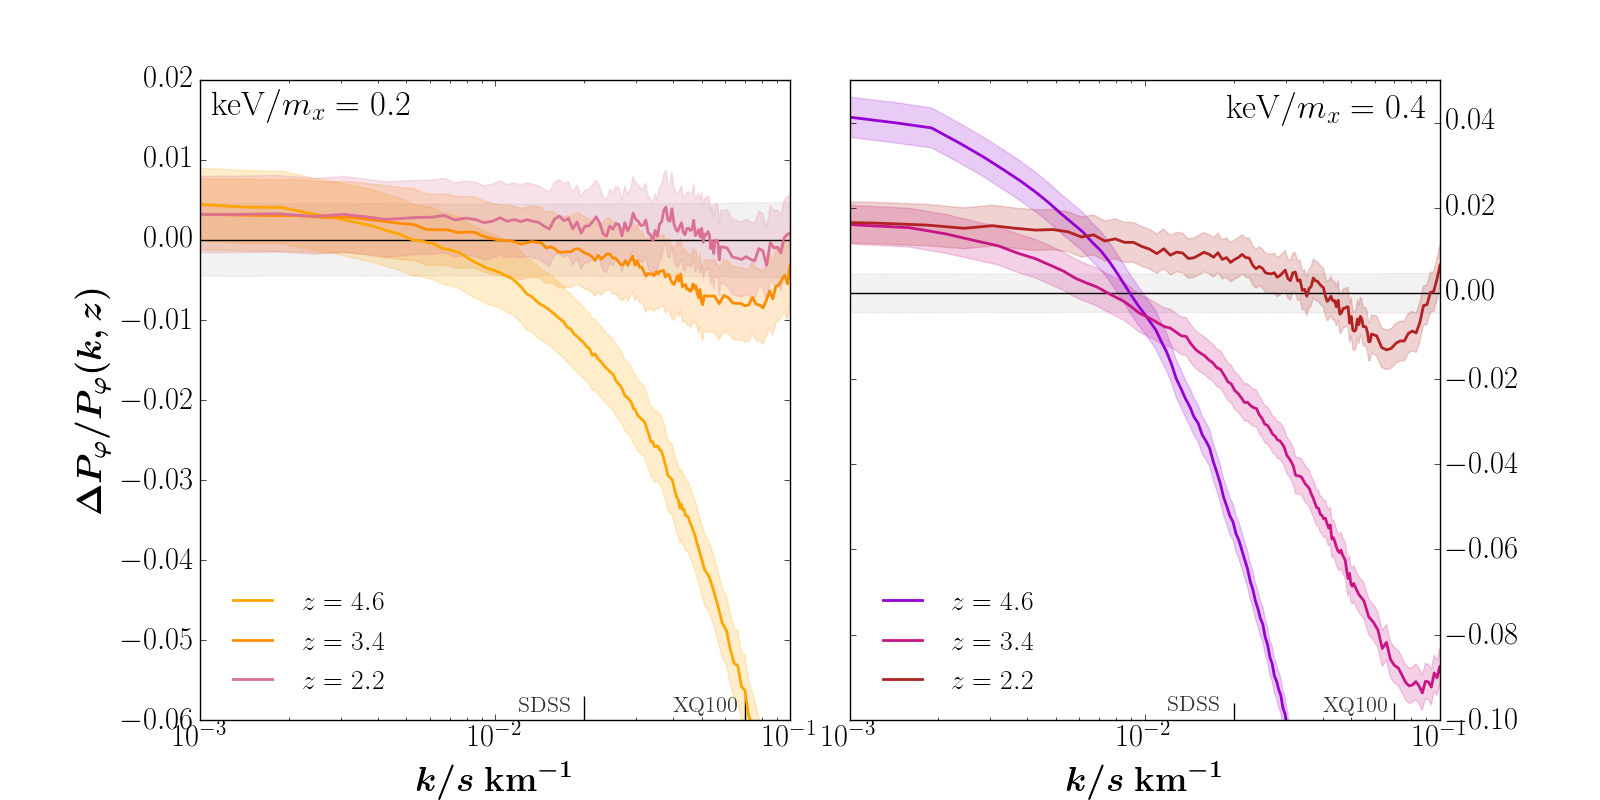
\includegraphics[width=0.75\columnwidth]{Figures/WDM/Mx_Pf.png}
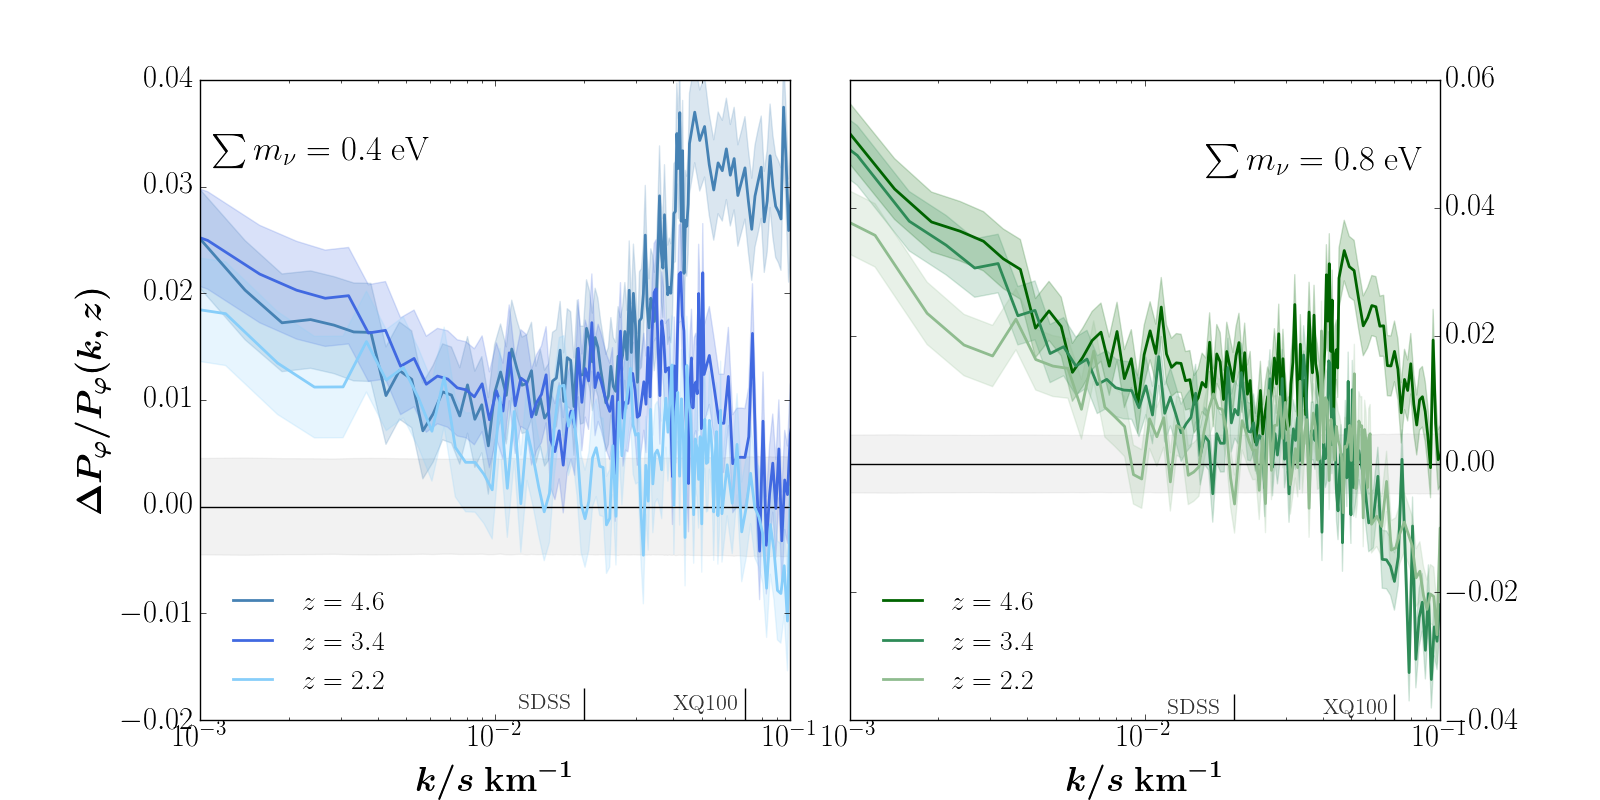
\includegraphics[width=0.75\columnwidth]{Figures/Mnu/Mnu_Pf.png}
\caption{Différence relative du spectre de puissance du flux Ly-$\alpha$ par rapport au modèle central (sans neutrinos, en trait noir) à 3 redshifts. L'épaisseur quantifie l'incertitude sur $P_\varphi$ dans les simulations numériques.}
\label{fig:pf}
\end{center}
\end{figure}

Les forêts Ly-$\alpha$ permettent de contraindre les paramètres cosmologiques à des échelles complémentaires à celles sondées par le fond diffus micro-ondes. En particulier, elles permettent de contraindre la masse des neutrinos à travers l'échelle caractéristique en-dessous de laquelle ils empêchent la formation de structures. Une amélioration de la résolution des simulations d'une part et une meilleure statistique de données d'autre part pourrait permettre la détection de la somme des masses positive des neutrinos dans les prochaines années, par exemple avec l'expérience DESI.